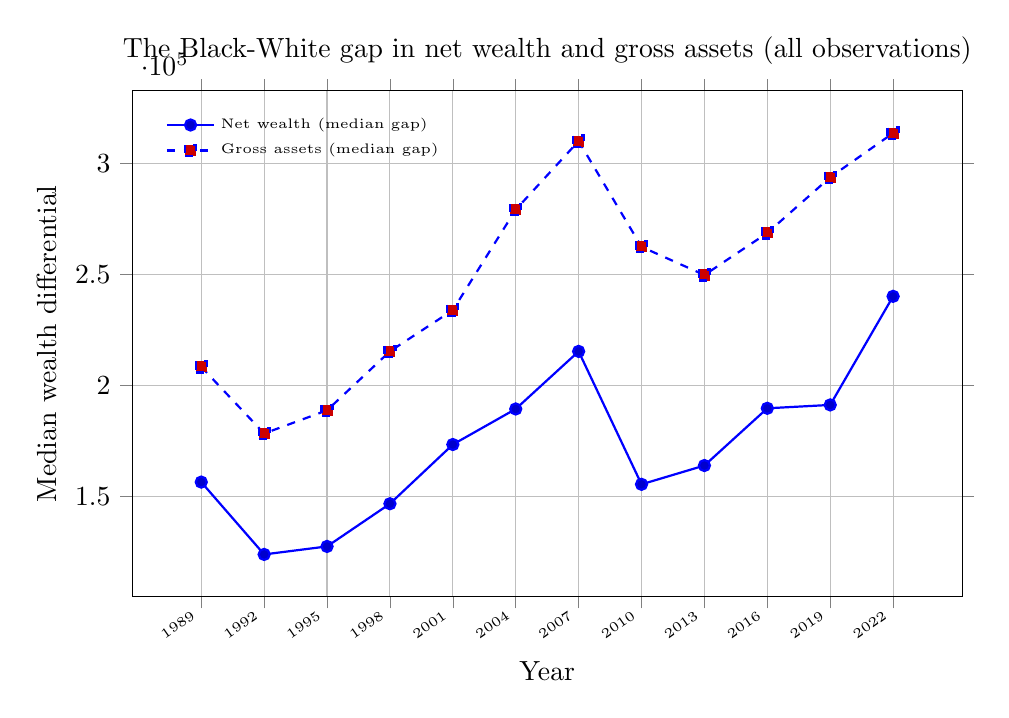
\begin{tikzpicture}
\begin{axis}[
width=\textwidth,
height=0.66\textwidth,
xlabel={Year},
ylabel={Median wealth differential},
title={The Black-White gap in net wealth and gross assets (all observations)},
legend pos=north west,
legend style={font=\tiny,draw=none,fill=none,cells={anchor=west}},
grid=major,
tick align=outside,
xtick={1989,1992,1995,1998,2001,2004,2007,2010,2013,2016,2019,2022},
scaled x ticks=false,
xticklabel style={/pgf/number format/fixed,/pgf/number format/precision=0,/pgf/number format/1000 sep={},rotate=35,anchor=east,font=\tiny},
]
\addplot+[thick, blue] coordinates {(1989, 156503.09799760) (1992, 123903.78788000) (1995, 127505.91773900) (1998, 146741.86666300) (2001, 173432.89977500) (2004, 189448.58886900) (2007, 215394.21844600) (2010, 155495.50562100) (2013, 163966.35253500) (2016, 189754.11499900) (2019, 191268.87416800) (2022, 240210.00000000)};
\addlegendentry{Net wealth (median gap)}
\addplot+[thick, blue, dashed] coordinates {(1989, 208424.86828400) (1992, 178396.59091300) (1995, 188839.59310200) (1998, 215426.83333700) (2001, 233983.74904100) (2004, 279262.64990800) (2007, 310169.39175400) (2010, 262505.36828800) (2013, 249818.94124500) (2016, 268763.85569400) (2019, 293858.54304300) (2022, 313770.00000000)};
\addlegendentry{Gross assets (median gap)}
\end{axis}
\end{tikzpicture}
